\documentclass[a4paper, 11pt]{article}

\usepackage[utf8]{inputenc}
\usepackage[T1]{fontenc}
\usepackage[francais]{babel} 
\usepackage{amsmath} % pour les formules de maths
\usepackage{amssymb} % pour des symboles
\usepackage{mathrsfs} % pour avoir acces a des jolies lettres calligrafiées. :)
\usepackage{listings} % pour le code source
\usepackage{color} % pour les couleurs
\usepackage{graphicx} % pour les graphiques (images)
\usepackage{fancyhdr} % pour utiliser le pagestyle fancy
\usepackage[headheight=14pt]{geometry} % pour les marges

\geometry{hmargin=3cm}

\title{Metaheuristics for Optimization\\SERIES 1 : NK-LANDSCAPE MODELS}
\author{Romain Mencattini}
\date{\today}

\pagestyle{fancy} % pour avoir des entetes et des pieds de page
\renewcommand\headrulewidth{0.6pt}
\fancyhead[L]{Romain Mencattini} % haut de page gauche
\fancyhead[R]{Université de Genève \today} % haut de page droite

\begin{document}
\maketitle
\newpage
\tableofcontents
\newpage

\section{Introduction}
\paragraph{}
Le but de ce tp est de pratiquer le problème des \textit{NK-landscape models}. Plus particulièrement de voir l'effet qu'à la modification
du paramètre $K$ sur les résultats. Le dit paramètre sert à modifier la \textit{rugosité}. On va donc utiliser deux méthodes: une
déterministe et une probabiliste. Pour chacune de ces méthodes, on va faire varier le $K$ avec:
\begin{center} $K = 0$\\ $K = 1$ \\ $K = 2$ \end{center}

On pose que $x$ est un vecteur de taille $N$ :\\
\begin{center} $x = (x_1,x_2,... ,x_N)$ avec $x \in \{0,1\}$ \end{center}

Il nous faut également une fonction de coût définie comme suit:
\begin{center} $F(x) = \sum\limits_{i=1}^{N-K} f_K (x_i,...,x_{i+K})$\end{center}

On va donc faire correspondre des groupes de bits de taille $K$ à une valeur $\in \mathbb{N}$ selon ce tableau donné dans le tp1:
\begin{center}

\begin{tabular}{c | c | c}
\  & 0 & 1 \\
\hline
$f_0$ & 2 & 1
\end{tabular}
\end{center}

\begin{center}
\begin{tabular}{c | c | c | c | c }
 \  & 00 & 01 & 10 & 11\\
 \hline
 $f_1$ & 2 & 3 & 2 & 0
\end{tabular}
\end{center}

\begin{center}
\begin{tabular}{c | c |c | c|c|c|c|c|c}
 \  & 000 & 001 & 010 & 011 & 100 & 101 & 110 & 111\\
 \hline
 $f_2$ & 0 & 1 & 1 & 0 & 2 & 0 & 0 & 0
\end{tabular}
\end{center}

Il nous reste à définir les voisins. Le voisinage d'un $x$ est l'ensemble de tout ses voisins.
Où un voisin est une chaîne de bits de la même taille que $x$, mais ayant un seul bit de différent par rapport à $x$.
\\
Pour différencier deux solutions, nous allons utiliser la distance de Hamming, qui calcule le nombre de bits qui diffèrent entre deux
résultats. 

\section{Hill-Climbing déterministe}
\subsection{Algorithme}
\paragraph{}
Pour cet algorithme, on prend toujours la meilleure solution. 
Par meilleure solution, nous entendons qu'une fois que les voisins ont été trouvés, on choisit toujours celui avec la meilleure fonction 
de coût : i.e.
\begin{center}
 $max(F(y))\  \forall y$ où $y \in V(x)$ 
\end{center}
Voici comme procède l'algorithme:
\begin{enumerate}
 \item génération d'une solution aléatoire de taille $N$
 \item génération des voisins
 \item choix du voisins qui permet de maximiser $F(x)$
 \item changement de la solution pour le voisin

\end{enumerate}

L'algorithme s'arrête lorsque plus aucun voisin ne permet d'augmenter $F(x)$. Il s'agit donc d'un algorithme glouton car on prend toujours
la meilleure solution jusqu'à arrêt du programme.

\subsection{Résultats}
\paragraph{}
Voici les trois histogrammes obtenus pour chaque valeur de $K$. Nous avons procédé à 50 lancements pour valeurs.

\paragraph{}
Pour $K=0$:\\
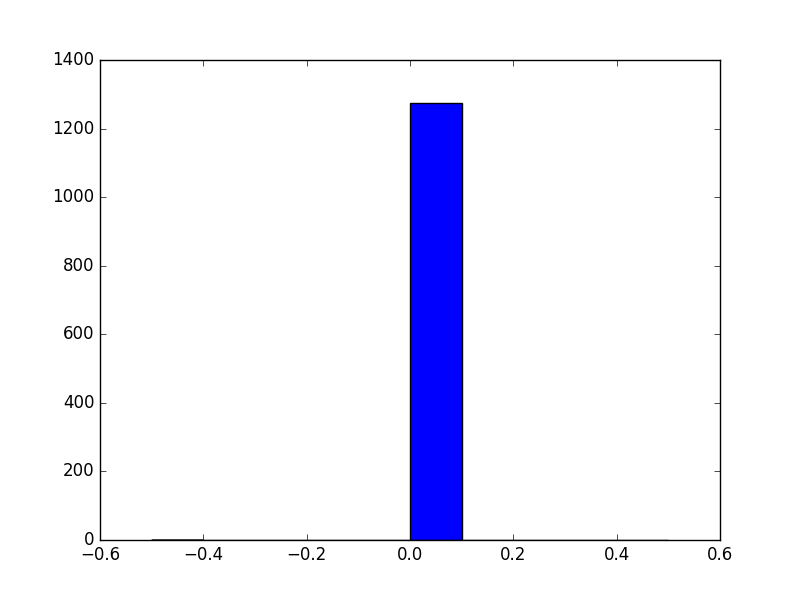
\includegraphics[scale=0.5]{d_d_0}
\\
On remarque qu'il n'y a aucune rugosité pour ce graphique. En effet, l'algorithme trouve à chaque fois la même solution. La distance de 
Hamming est donc nulle dans tout les cas.

\paragraph{}
Pour $K=1$:\\
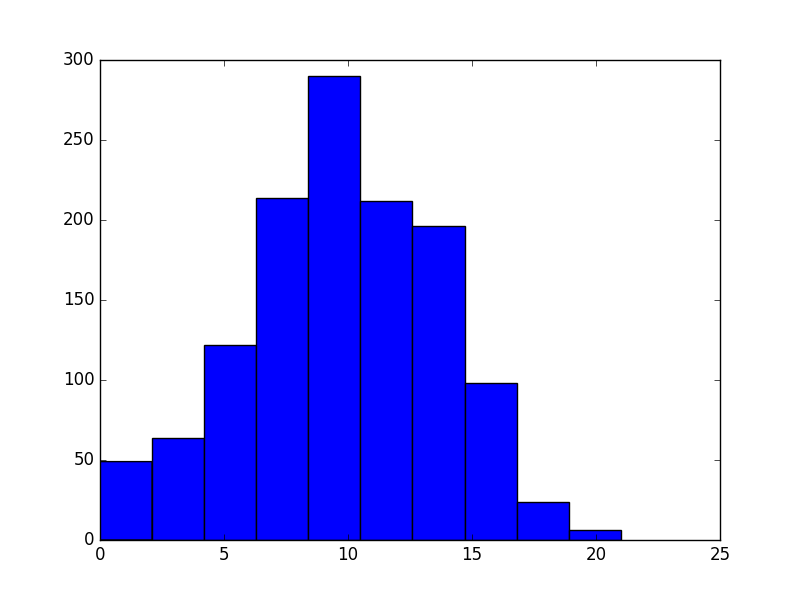
\includegraphics[scale=0.5]{d_d_1}
\\
Dans ce cas-ci, il y a plus de rugosité. On voit apparaître une loi normale centrée en 10. On a donc une majorité de résultats qui se 
trouvent au centre. Il y a peu d'histogrammes qui se trouvent très éloignés du centre. Donc une variance peu élevée.

\paragraph{}
Pour $K=2$:\\
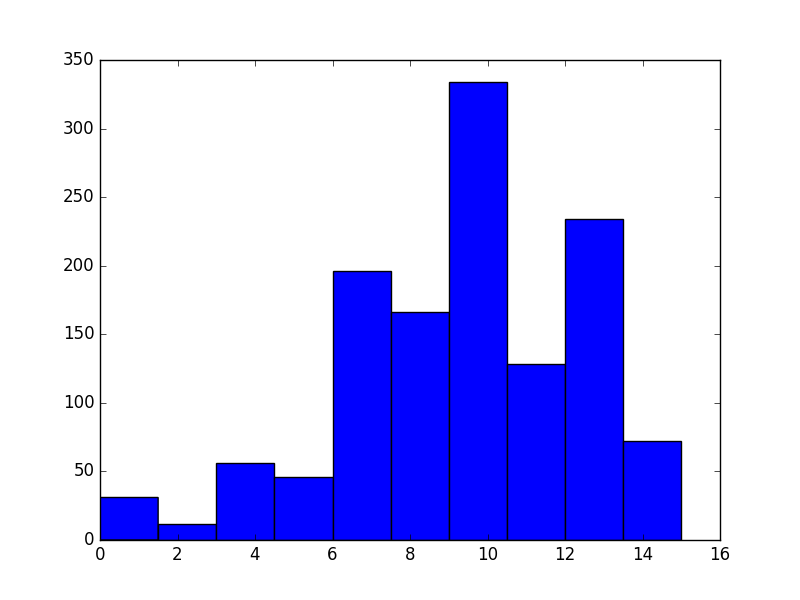
\includegraphics[scale=0.5]{d_d_2}
\\
Cette fois-ci, on remarque qu'il y a une très grande rugosité. Il n'y a pas de loi normale, Les histogrammes sont répartis sur presque 
toute la largeur avec des hauteurs variable. Il y a donc énormément de solutions différentes trouvées par le programme déterministe.
On peut supposer qu'il y a de nombreux maximas locaux et que la version déterministe tombe dedans souvent.

\section{Hill-Climbing probabiliste}
\subsection{Algorithme}
Dans cette version l'idée est un peu différente. En voici le déroulement:
\begin{enumerate}
 \item on génère une solution aléatoire
 \item on génère les voisins
 \item on associe une probabilité aux voisins
 \item on regarde s'il y a un voisin qui permet d'améliorer le meilleur résultat qu'on a eu et on revient au point 2.
 \item si le 4. n'est pas vérifié on choisit (en tenant compte des probabilités) un voisin parmi ceux présents
\end{enumerate}
La condition d'arrêt est d'avoir effectué un certain nombre d'itération. On choisit empiriquement de le fixer à dix fois le nombre
d'étapes nécessaires pour trouver une solution avec la version déterministe (en moyenne).

\paragraph{}
Les probabilités sont calculées comme étant la valeur de $F(x)$ divisée par la somme de toutes les $F(x)$.

\paragraph{}
Avec cet algorithme, il est possible de choisir des solutions moins bonnes. Mais cet inconvénient permet de ne pas rester coincer dans des 
minimas locaux.
On a aussi une "intention" qui ; si on trouve une solution meilleure que toutes les précédentes, nous la fait choisir pour tenter de
nous "indiquer" le chemin jusqu'à la solution optimale.
On est sûr que si on laisse tourner l'algorithme un temps infini, on va forcément trouver le maxima global, ce qui n'est pas le cas avec
la version déterministe.

\subsection{Résultats}

\paragraph{}
Pour $K=0$:\\
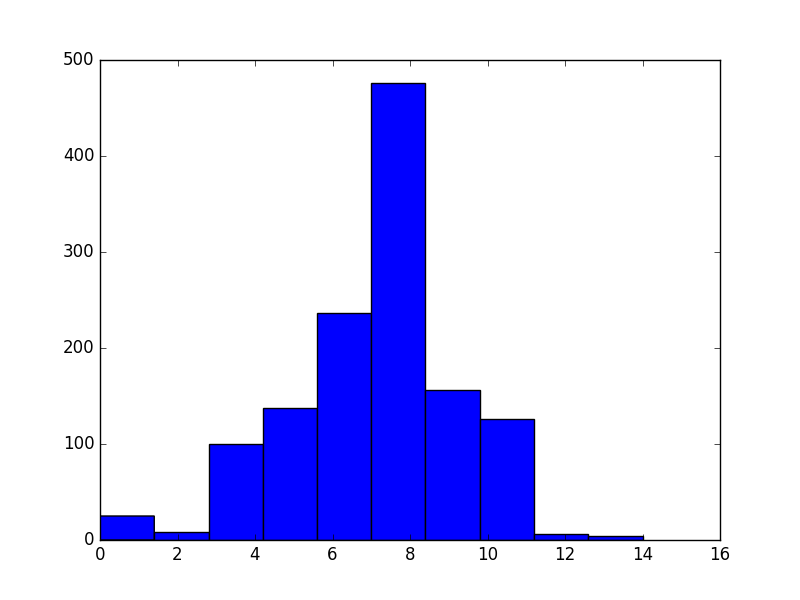
\includegraphics[scale=0.5]{d_p_0}
\\
On voit un histogramme qui est bien plus représenté que les autres. Cependant c'est moins net que pour le déterministe. On n'a pas 
effectué assez de pas pour lisser le graphe.

\paragraph{}
Pour $K=1$:\\
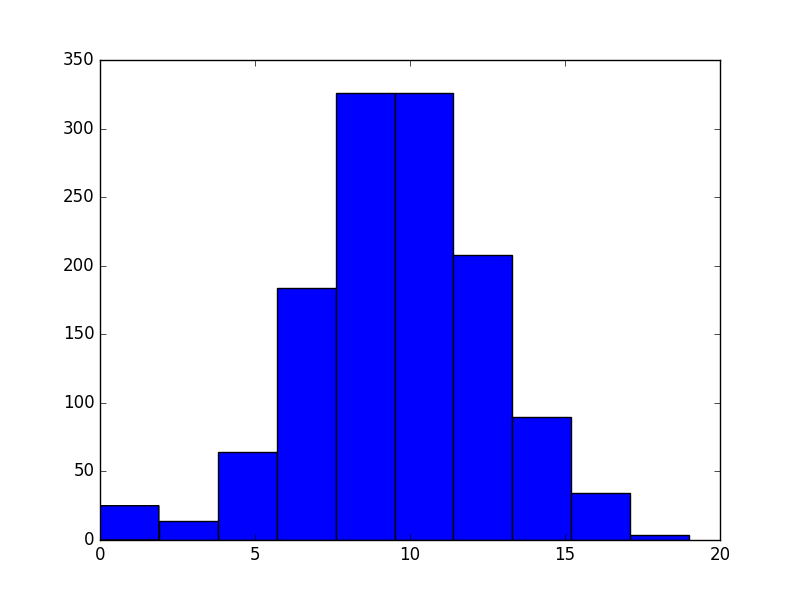
\includegraphics[scale=0.5]{d_p_1}
\\
Dans ce cas-ci, les résultats sont ,encore une fois, moins bon que pour la version avec $K=0$. On voit néanmoins que les résultats sont 
plus uniformes que pour la version déterministe. Il y a donc moins de résultats différents car les probabilités poussent les réponses à
se ressembler.

\paragraph{}
Pour $K=2$:\\
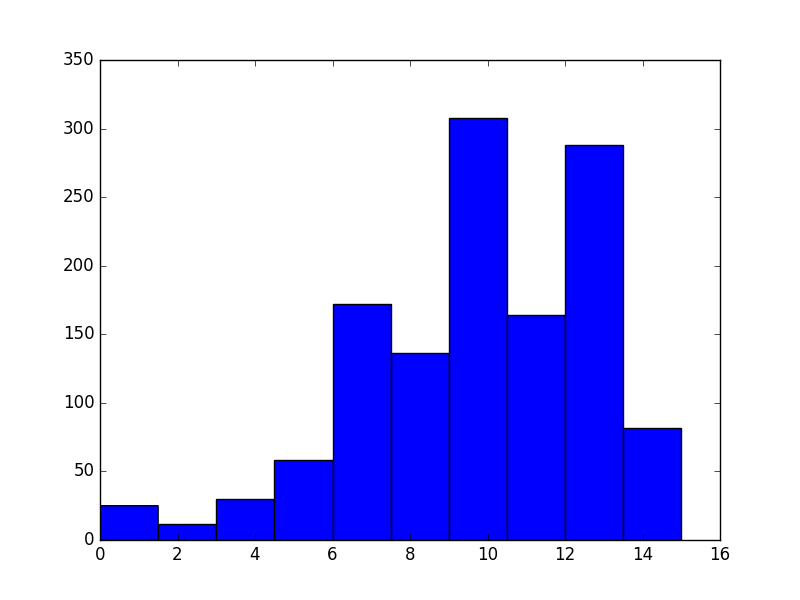
\includegraphics[scale=0.5]{d_p_2}
\\
Les résultats sont très chaotiques comme pour la version déterministe.

\section{Conclusion}
\paragraph{}
On remarque avec les histogrammes que le fait d'augmenter $K$ rend les solutions moins uniformes, plus aléatoire. Les graphes sont
plus rugueux. 
Il est intéressant de noter que la version probabiliste pour $K=1$ est moins rugueuse que la version déterministe. Nous pensons que 
cela est dû aux probabilités et à l'intention qui dirigent les solutions dans le même sens.
\paragraph{}
Pour $K=0$, nous n'avions qu'une seule solution optimale et aucun maximas locaux: celle avec que des $0$. Dans le cas de $K=1$ et $K=2$,
il y a des maximas locaux, ce qui se traduit par des résultats moins uniformes.
Concernant la version probabiliste, le choix de ne pas toujours choisir la meilleure solution la pénaliser pour $K=0$.

\end{document}